\chapter{TSP 渗透测试与远程入侵}
\label{ch5}
\section{攻击模型}
实验环境包括某知名品牌汽车一台,装有远程控制 App 的手机一部,无线路由
器一个以及一台装有无线网卡的电脑。软件环境:手机环境为安卓5.9.1,手机智能互联APP)。汽车已经具有网联远控的功能,在第四章对其进
行威胁建模的基础上,对其进行实际攻击测试,证明当前的 ICV 领域确实还存在很
多不容忽视的安全问题。
\begin{figure}
    \centering
    
\includegraphics[scale=0.5]{resources/img/i14.png}
    \caption{网络图片非真实测试车}
  \end{figure}
\newline
整体的流程如图 5.2 所示。大致分为环境搭建、数据分析、漏洞利用和逆向工程
几个步骤,与后文的章节基本上是相互对应的。实验用车经过多次测试,已经确定
存在相关漏洞;首先在近距离通信使用蓝牙伪造请求攻击, 具体来说首先分析蓝牙协议配对握手协议,然后通过抓取蓝牙通信打印文件, 在打印文件中找到对应指令操作请求
通过同一局域网PC进行伪造请求 从而达到远程控制智能网联汽车的目的;在逆
向工程部分,对 App 进行初级反编译,找出可能存在的加固方式,然后使用动态方
式 Dump 内存中的 DEX 文件,再进行反汇编和动态调试,从汇编代码中找到指令以
及服务器的认证格式;最后用相应的代码进行验证。
\begin{figure}
  \centering
  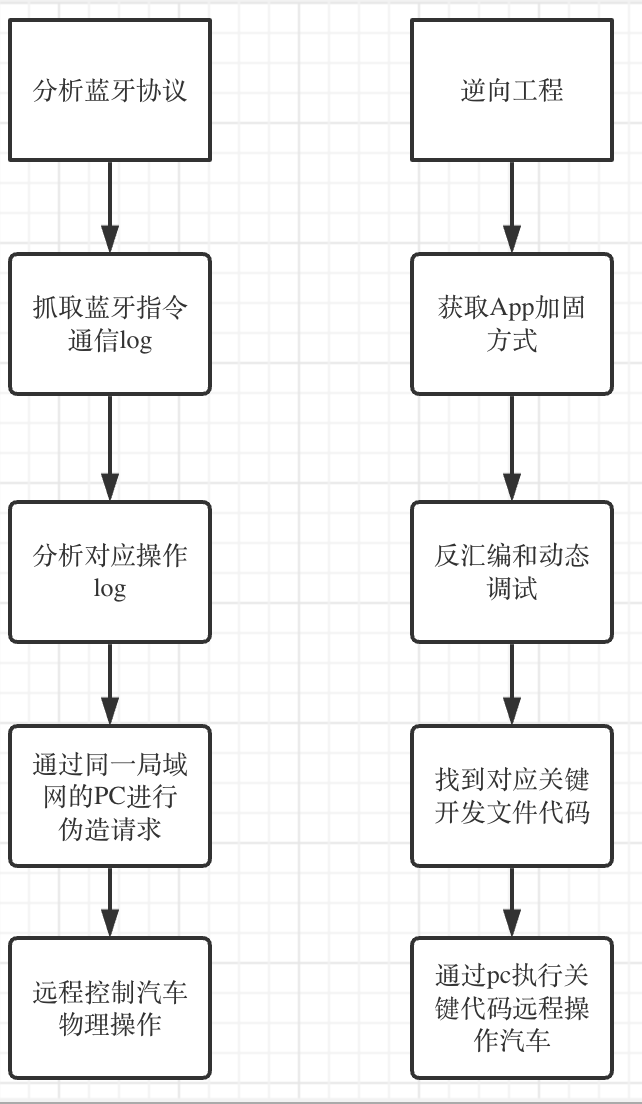
\includegraphics[scale=0.5]{resources/img/i23.png}
  \caption{漏洞挖掘和攻击步骤图}
\end{figure}
\newline
\section {蓝牙近距离通信漏洞利用}
蓝牙作为一种近距离数据交换的通信方式,也
是恶意攻击者关注的一个攻击面。攻击者能够利用
蓝牙接口在汽车的信息娱乐单元上执行恶意代码,
从而实现对车辆内部网络的渗透和攻击。文献\cite{antian}
利用蓝牙漏洞,开发出一款名为“BlueBorn”的攻
击向量,实现了对IVI系统的控制。
近年来某些汽车厂商实现了所谓“蓝牙钥匙”的功能:
使用汽车App开启手机钥匙后,手机便可以取代随车的遥控钥匙,进行解锁、上锁和启动车辆等操作。
这里我们实现了通过伪造传输数据,恶意控制汽车行为。

\subsection{蓝牙通信前置知识}
简单地说,蓝牙是一种短程宽带无线电技术,是实现语音和数据无线传输的全球开放性标准。它使用跳频扩谱(FHSS)、时分多址(TDMA)、码分多址(CDMA)等先进技术,在小范围内建立多种通信与信息系统之间的信息传输。

蓝牙使用跳频技术,将传输的数据分割成数据包,通过79个指定的蓝牙频道分别传输数据包。每个频道的频宽为1 MHz。蓝牙4.0使用2 MHz 间距,可容纳40个频道。第一个频道始于2402 MHz,每1 MHz一个频道,至2480 MHz。有了适配跳频(Adaptive Frequency-Hopping,简称AFH)功能,通常每秒跳1600次。

最初,高斯频移键控(Gaussian frequency-shift keying,简称GFSK)调制是唯一可用的调制方案。然而蓝牙2.0+EDR 使得 π/4-DQPSK和 8DPSK 调制在兼容设备中的使用变为可能。运行GFSK的设备可以以基础速率(Basic Rate,简称BR)运行,瞬时速率可达1Mbit/s。增强数据率(Enhanced Data Rate,简称EDR)一词用于描述π/4-DPSK 和 8DPSK 方案, 分别可达2 和 3Mbit/s。在蓝牙无线电技术中,两种模式(BR和EDR)的结合统称为"BR/EDR射频"。

蓝牙是基于数据包、有着"主从架构"的协议。一个主设备至多可和同一网域中的七个从设备通讯。所有设备共享主设备的时钟。分组交换基于主设备定义的、以312.5µs为间隔运行的基础时钟。两个时钟周期构成一个625µs的槽,两个时间隙就构成了一个1250µs的缝隙对。在单槽封包的简单情况下,主设备在双数槽发送信息、单数槽接受信息。而从设备则正好相反。封包容量可长达1、3、或5个时间隙,但无论是哪种情况,主设备都会从双数槽开始传输,从设备从单数槽开始传输。
如图5.4
这里简短的说下蓝牙协议的类型: 
其实我们蓝牙协议主要分为传统蓝牙和低功耗蓝牙。

对于传统蓝牙来讲,当提出主动连接的设备(搜索设备)和被连接的设备(被搜索设备)打算进行连接时,搜索设备会以极快的速度进行跳频,被搜索设备会以极低的速度跳频,这样两个设备一定会同时跳跃到同一频段(79个频段中的一个)。

随后,搜索设备和被搜设备进行连接,并会将连接信道按照跳频图(由发起连接的设备)进行有规律的变化。当中,发起连接的一方被称为Master,接受连接的一方称为Slave此外,在建立连接后,双方根据已建立逻辑、基于 BR/EDR controller的l2cap 可以沟通各自是否具备可以使用的Altemate的AMP Controllers,具备的话则会判定是否将传输的data,转移到这些Controllers(极大提供蓝牙传输效率)。

对于低功耗蓝牙来讲,同样存在两方,称为Adversting的一方,发 送adversting packets(广播包),接收的一方称为Scanner,当Scanner接受到 "connectable advertisingpacket" 回应 "connection request"  建立起点对点链接(Initiators),Initiators发起连接即为Master ,Scanner为Slave。频道的选择则是在有Master生成的Hopping Pattern决定。
这里解释下几个专用名词:
\begin{itemize}
    \item SMP SMP即安全管理协议,为BLE设备提供建立加密连接需要的key(STK or LTK)。位于L2CAP 与 GAP之间 为消息传递进行了安全加密。将生成加密key的过程称为Pairing(配对),并详细定义了Pairing的概念、操作步骤、实现细节等。定义一个密码 工具箱(CryptographicToolbox),其中包含了配对、加密等过程中所需的各种加密算法。定义一个协议(SecurityManager Protocol,简称SMP),基于L2CAP连接,实现master和slave之间的配对、密码传输等操作。
    \item L2CAP Protocol 在 用户类XXX-U Logical Link的基础上,抽象出和具体技术无关的数据传输通道(包括单播和广播两类),L2CAP channel endpoints的概念(类似TCP/IP中的端口),为具体的应用程序(profile)提供独立的数据传输通道。在构建了点对点的逻辑通道,将这个 LogicalChannel换为L2CAP Channel,实现逻辑信道复用和长数据的分片传输
    \item ATT(Attribute Protocol : 最终生成STK用户建立加密连接,建立加密连接后再自行生成LTKS,通过Transport Specific Key Distribution共享双方生成EDIV和Rand用于索引LTK
    \item LTK:长期密钥
    \item IRK:身份解析密钥   当私有地址周期性变化时可通过IRK并依据list对周期性变化的地址向MAC地址映射(BLE地址随机性)
    \item CSRK:连接签名解析密钥  连接使用数据签名来保护连接(其提供了完整性和认证)
\end{itemize}


\begin{figure}
    \centering
    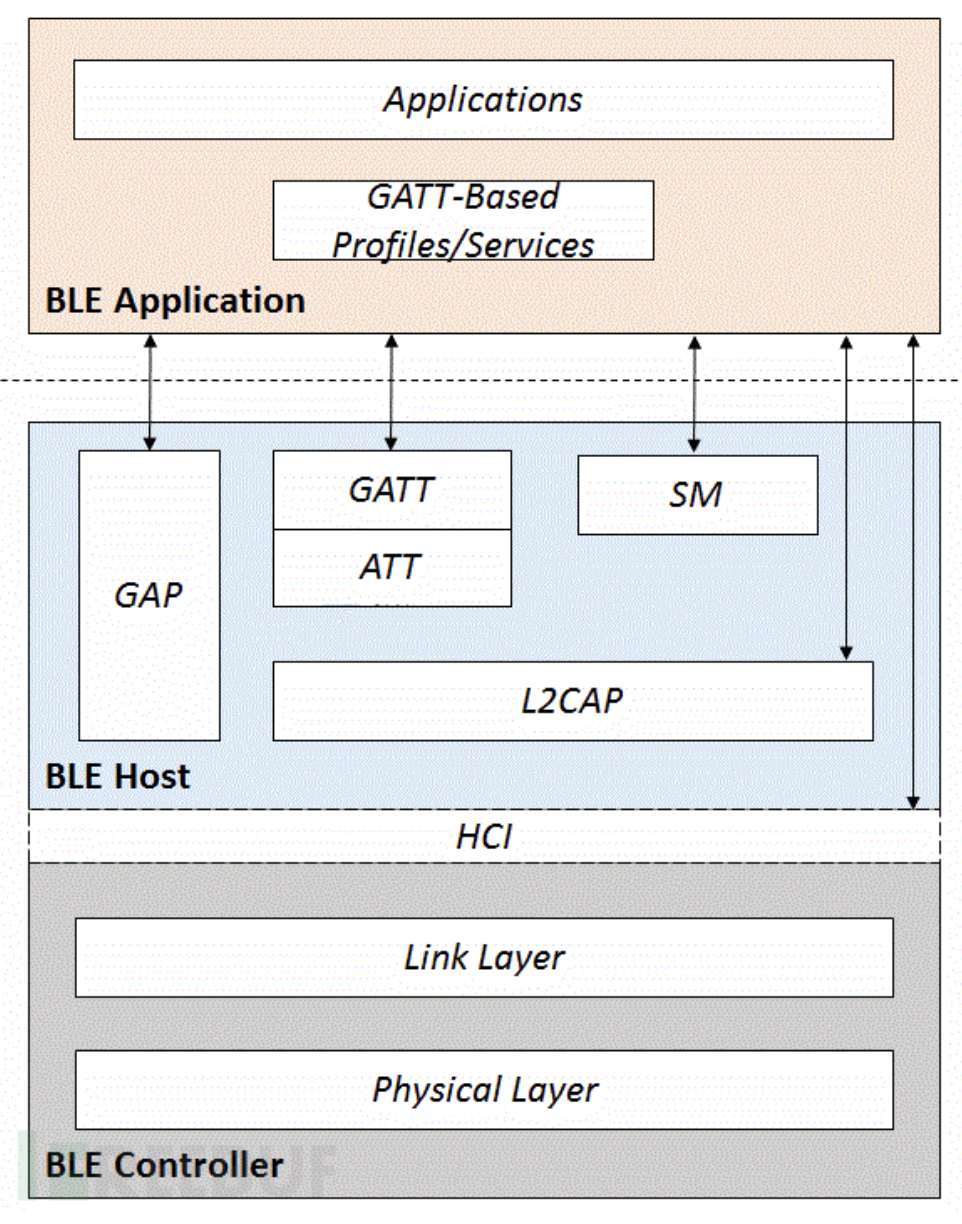
\includegraphics[scale=0.5]{resources/img/i15.png}
    \caption{蓝牙握手协议示意图}
  \end{figure}

\subsection{蓝牙协议配对流程}
\begin{itemize}
    \item 配对发起者(Initiator,总是Master)和配对的回应者(Responder,总是Slave)可以交换足够的信息,以决定在阶段2使用哪种配对方法、哪种鉴权方式。
    配对方法:LE legacy pairing 和 LE Secure Connections(新方法优先支持)
    \item 鉴权 如果双方都支持OOB鉴权,则选择该方式(优先级最高)否则,如果双方都支持MITM鉴权,则根据双方的IO Capabilities(并结合具体的配对方法),选择合适的鉴权方式
    \item 获取密钥: 最终生成STK用户建立加密连接,建立加密连接后再自行生成LTKS,通过Transport Specific Key Distribution共享双方生成EDIV和Rand用于索引LTK
\end{itemize}

当我们都配置好了就可以手机汽车app抓包了。运行手机汽车互联app就可以被fiddler所截取到数据包了。
通过检测配对的蓝牙协议中,并未发现使用SMP,所以BLE模块和APP之间并不会进行安全的权鉴, 如图5.6
\newline
\subsection{通过蓝牙实现伪装请求攻击}
具体攻击思路如下\cite{von2021method}:
\begin{itemize}
    \item 让安卓设备抓取到发送的信息
    \item 拿到蓝牙信息进行wine shark 过滤出关键信息
    \item 让电脑设备的linux进行数据读写,达到蓝牙操控的目的
\end{itemize}

(1) 安卓设备首先获取root权限进入文件目录,在设备里进入蓝牙目录,找到bt\_stack.conf蓝牙配置文件,然后在在开发者选项里打开蓝牙HCI信息收集日志
此时若继续蓝牙收发数据可观测到控制台出现了/btsnoop\_hci.log文件,这里有我们所需要的打印信息,如图5.5

(2) 通过adb 命令进行手机的连接,导出我们的.log 文件
\begin{figure}
    \centering
    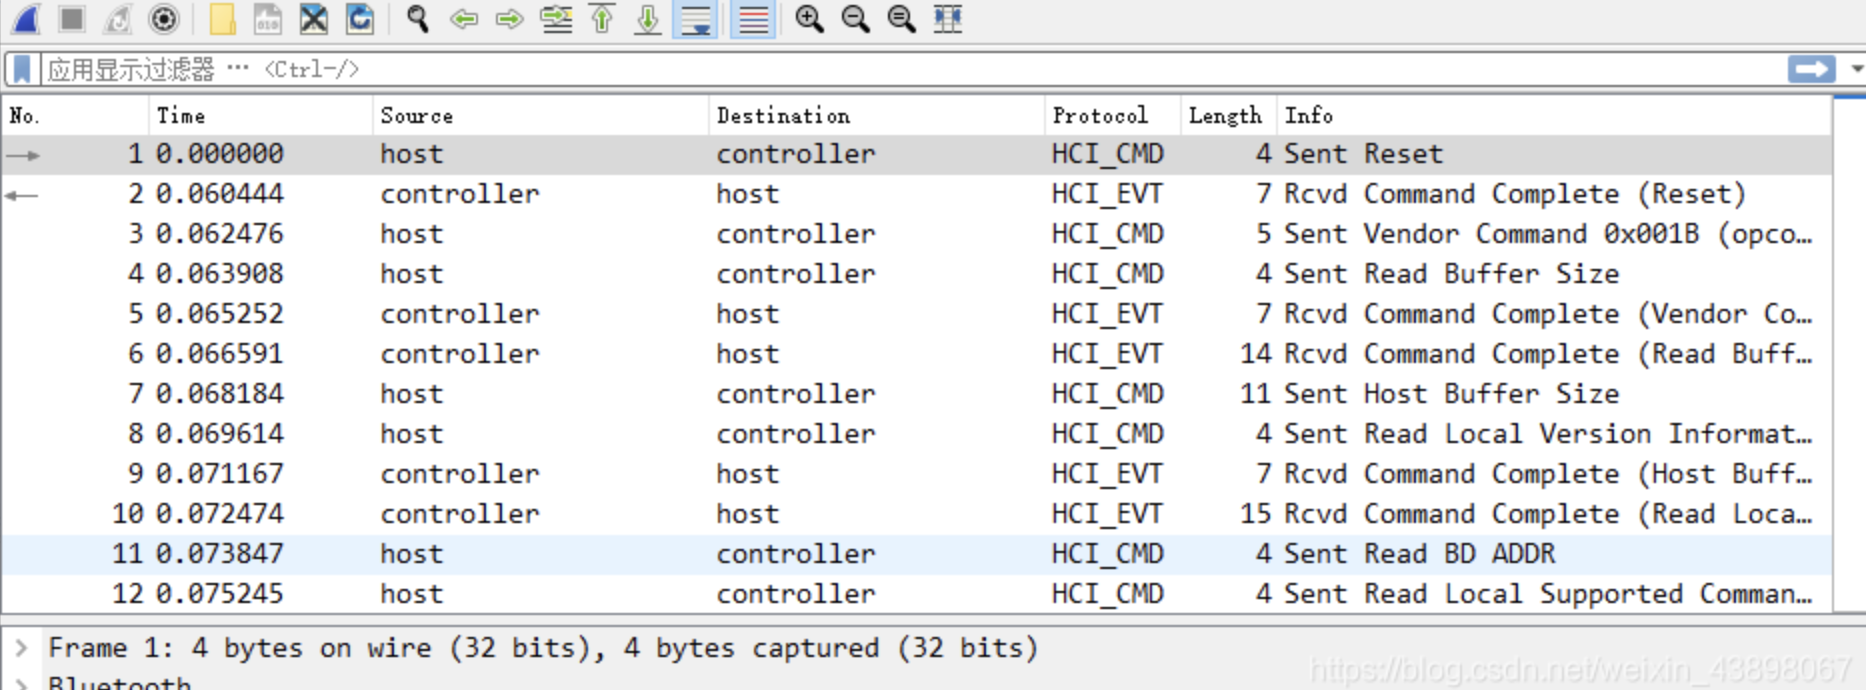
\includegraphics[scale=0.5]{resources/img/i17.png}
    \caption{蓝牙传输数据打印文件图}
  \end{figure}
(3) 通过从手机设置里找到对应的mac地址 我们通过工具过滤出来该设备的蓝牙传输信息。
  
当我们在手机APP下发"开锁"命令时:通过打印工具发现发现:
对应Handle字段为:'0x0019',value是: 313233,
当我们在手机APP下发"解锁"命令时:通过打印工具发现:
对应Handle字段为:'0x004e',value是: 000000。
\begin{figure}
    \centering
    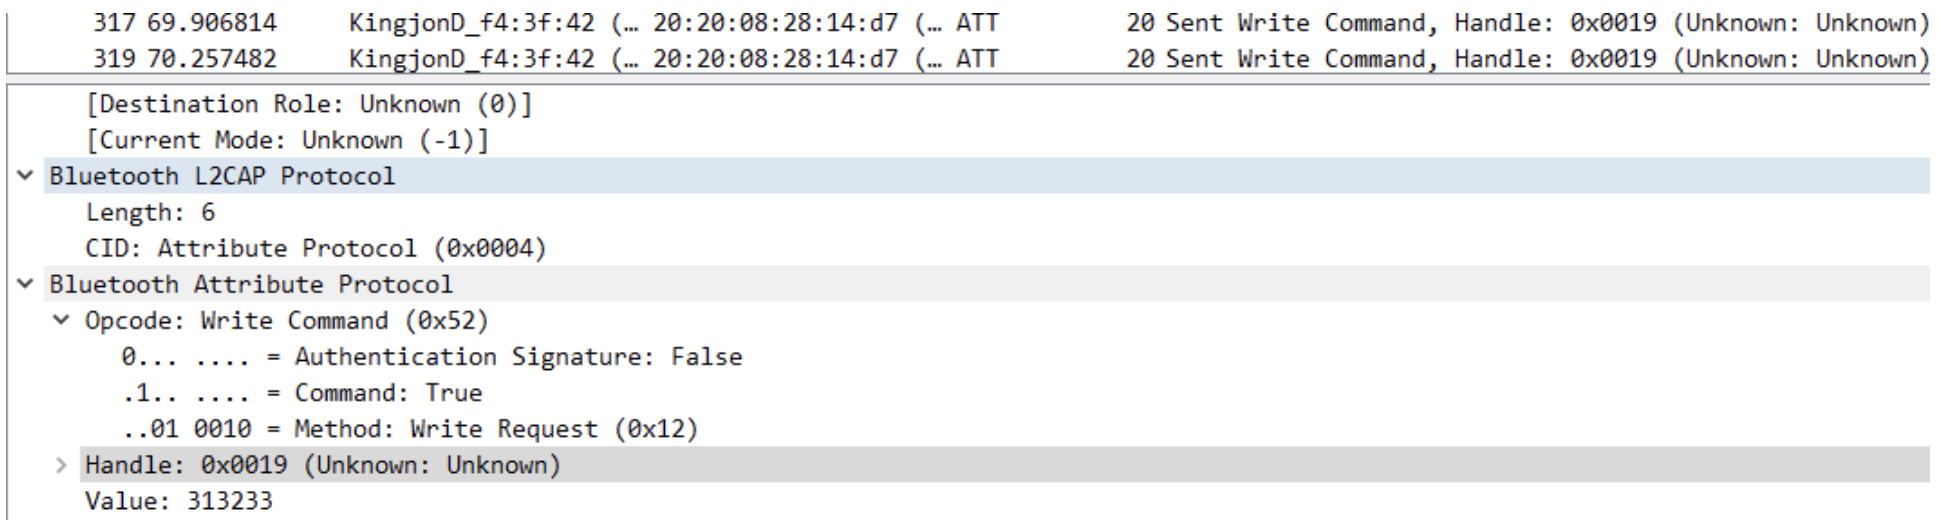
\includegraphics[scale=0.5]{resources/img/i18.png}
    \caption{蓝牙对应操作数据字段图}
  \end{figure}
根据对应字段参数规则,我们可以伪造请求参数\cite{lu2005conditional},
任意的通过pc给配对中的智能网联汽车发送操作指令
从而达到远程恶意控制该智能网联汽车的目的。
此外经过研究和攻击我们还可以通过蓝牙协议对该智能网联汽车进行更多危险的操作。
\begin{figure}
    \centering
    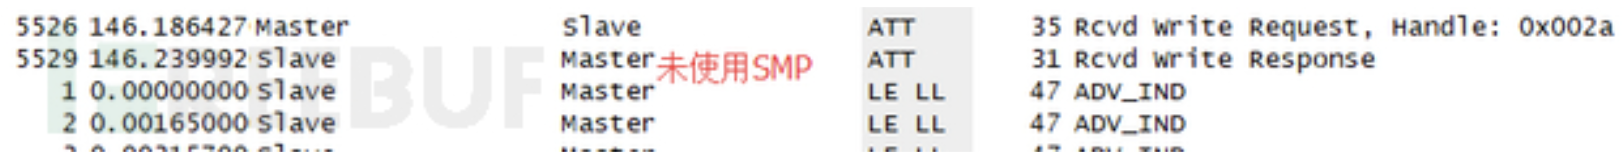
\includegraphics[scale=0.5]{resources/img/i16.png}
    \caption{蓝牙协议加密图}
  \end{figure}

\section{逆向工程APP和破解请求加密
}
关于车内 ECU 的逆向,这里重点放在对 TSP 系统中
客户端的逆向和破解。获取到 Cookie 和 Token ,我们就可以向汽车发送控制指令。但是,到目前为止,控制指令的格式无法知晓,也
无法通过简单的类比进行推断。较好的办法就是对 App 进行反编译\cite{yang2015automated}。Android 应用程
序包(APK)是一种可以在 Android 平台上运行的应用程序安装包,类似于 Windows
操作系统中的待安装 EXE 文件。很多 APK 由于进行了加固和代码混淆,无疑大大
增加了破解 App 的难度。

Android应用程序包(英语:Android application package,APK),是Android操作系统使用的一种应用程序包文件格式,用于分发和安装移动应用及中间件。
一个Android应用程序的代码想要在Android设备上运行,必须先进行编译,然后被打包成为一个被Android系统所能识别的文件才可以被运行,
而这种能被Android系统识别并运行的文件格式便是“APK”。 
一个APK文件内包含被编译的代码文件(.dex 文件),文件资源(resources), assets,证书(certificates),和清单文件(manifest file)。

\subsection{工具准备}
\begin{itemize}
    \item apktool:资源文件获取,可以提取出图片文件和布局文件进行使用查看。
    \item dex2jar:将APK反编译成Java源码(classes.dex转化成jar文件)。
    \item 查看APK中classes.dex转化成出的jar文件,即源码文件 下载apktool、dex2jar、jd-gui,完成后将三个文件放在同一文件中,并解压dex2jar、jd-gui压缩包,这一步是为了方便进行反编译。
\end{itemize}

\subsection{执行APK反编译}
\begin{figure}
    \centering
    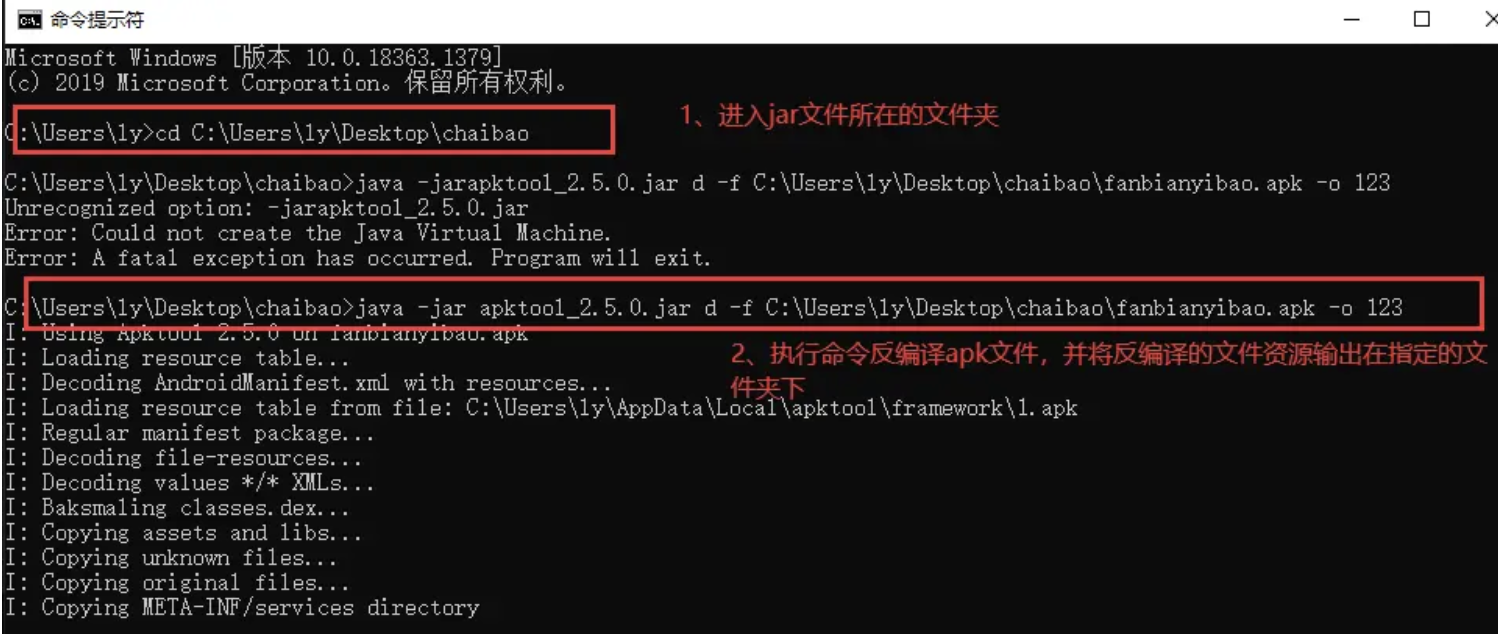
\includegraphics[scale=0.5]{resources/img/i19.png}
    \caption{反编译命令执行行图}
  \end{figure}

  \subsection{获取反编译成功后文件}
  打开对应的文件夹可以看到反编译后生成的文件,在这些生成的文件和文件夹当中,
  我们关心的是res文件夹中和AndroidManifest.xml文件,打开res文件夹,里面存放了我们所关心的xml文件,如图5.8所示:
  \begin{figure}
    \centering
    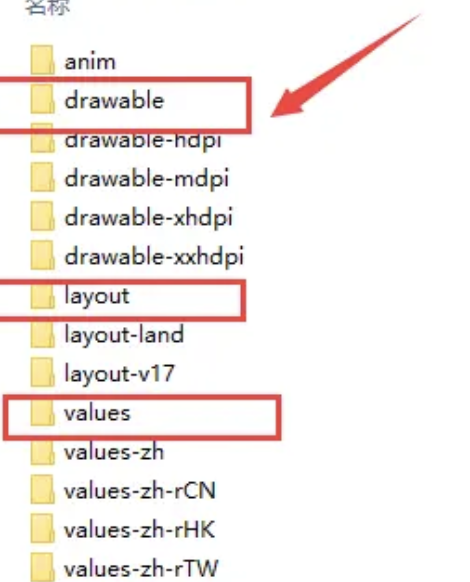
\includegraphics[scale=0.5]{resources/img/i20.png}
    \caption{apk开发文件列表图}
  \end{figure}
  图中展示了APK文件反编译后的资源文件,下面对这些文件做一个简单的介绍:
  \begin{itemize}
    \item META-INF:保存APP的签名信息。
    \item AndroidManifest.xml:Android清单文件,向Android系统提供应用的必要信息。
    \item classes.dex:.dex是Dalvik虚拟机上的可执行文件,需要使用dex2jar将其转换为jar文件。
    \item assets:存放一些资源文件字体,声音等。
    \item lib:存放第三方库。
    \item original:存放未经过反编译的等AndroidManifest.xml文件。
    \item res:存放资源文件,例如图片、颜色、字符等。
    \item smali:存放Java编译成的smali代码,smali相当于Android虚拟机上运行的语言。
\end{itemize}
\subsection{解析加固APK}
(1)APK 加固原理。在进行脱壳之前,我们需要简单了解一下 APK 的加固过
程。所谓 APK 加固也就是加壳,给目标 APK 加一层保护程序,隐藏 APK 敏感信
息。加壳程序可以有效防止黑客或者不法者对应用程序进行反编译和逆向分析。壳
本质的功能其实是实现类加载器。加壳后的 DEX, Android 虚拟机首先对其进行解密操作,再加载到系统内存中运行。
其中加壳过程如图 5.9 所示
在图中,简易的描述了加固的原理,首先我们会拿到一个需要加固的源apk文件,然后需要加固这个源apk,我们就会写一个对应的壳程序,
然后我们需要将两个apk合并,为了让程序能够正常运行,我们就需要将源apk文件和壳程序的dex文件进行合并,
然后用合并之后的dex文件将可程序的dex文件替换掉,这样我们的壳程序就会照成运行。
这里说明下什么是Dex文件:
我们都知道apk的本质是一个压缩包,当我们直接将.apk的后缀改为.zip的时候,是可以直接解压出里面的文件的(甚至有些压缩软件可以直接解压.apk文件,例如bindizip)。那么app为什么能在手机中运行呢,靠的就是.dex文件,
在Windows端的可执行文件是.exe文件,JVM的可执行文件是.class文件,那么在Android中的dalvik或art虚拟机上运行的可执行文件就是.dex文件。
\subsection{脱壳加固APK}
脱壳是把加在软件上的保护程序Dex去掉 直接能看到对应的源码。
跟java类似,安卓的class都是由Classloader的loadClass方法加载的。跟java不同的是,每一个class对象都会有对应的dex对象属性跟相应的dex文件关联起来。利用xposed,将loadClass方法劫持住,每当loadClass方法调用完成后,用xposed执行后置方法。获取方法加载的class对象,然后调用getDex方法。
拿到对应的dex文件引用,最后将dex文件序列成byte数据,写到自定义保存文件里面去。就能拿到脱壳后的dex文件。
我们通过"反射大师"这款软件来进行脱壳处理,其需要在 Xposed 环境中使用,支持市面上大多数加密壳。
\begin{itemize}
  \item 手机或模拟器安装xposed环境
  \item 安装反射大师,xposed内部勾选反射大师模块,重启模拟器。
  \item 打开目标app进入到主界面。
  \item 选择当前ACTIVITY长按写出Dex约两秒后释放,然后点击确定。dex文件可以直接拉到jadx查看源码
\end{itemize}

\begin{figure}
  \centering
  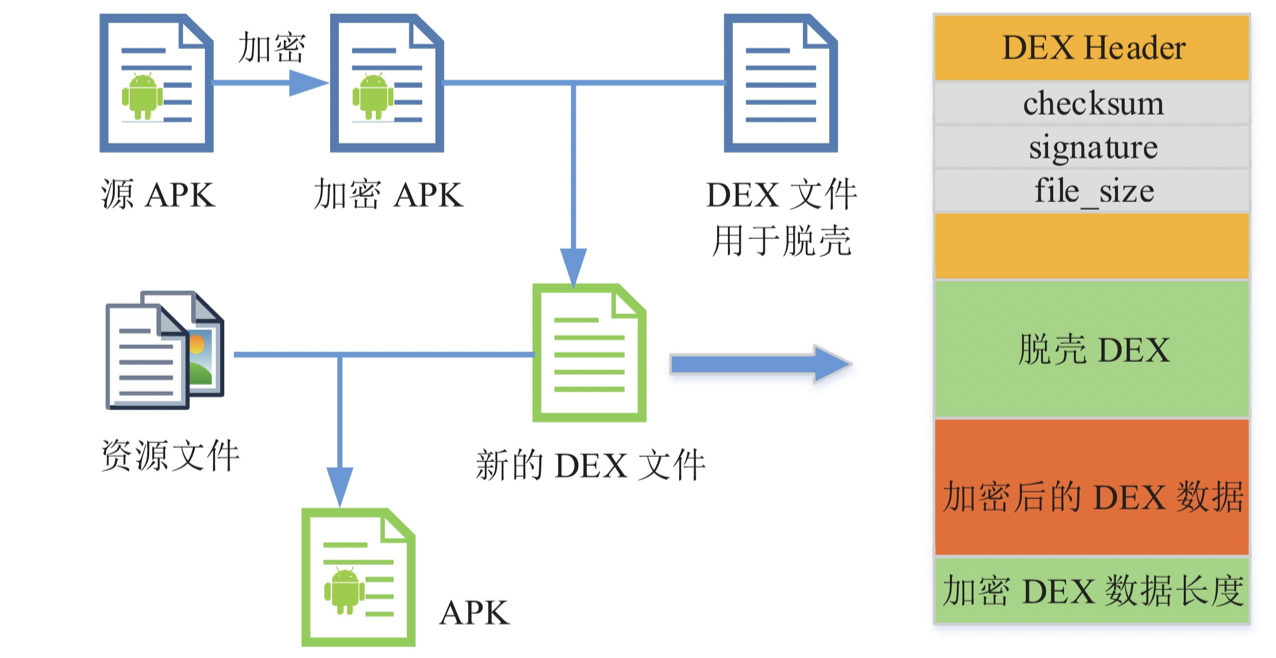
\includegraphics[scale=0.5]{resources/img/i24.png}
  \caption{目标APK加固分析}
\end{figure}

\subsection{分析关键操作代码}
\begin{lstlisting}[language=Java,title={获取汽车初始化地理位置代码}]
  private void initLocationStyle() {
    BitmapDescriptor descriptor = BitmapDescriptorFactory.fromResource(R.drawable.main_location_icon);
    MyLocationStyle myLocationStyle = new MyLocationStyle();
    myLocationStyle.myLocationIcon(descriptor);
    myLocationStyle.interval(2000); 
    myLocationStyle.myLocationType(MyLocationStyle.LOCATION_TYPE_FOLLOW);
    myLocationStyle.myLocationType(MyLocationStyle.LOCATION_TYPE_LOCATE);
    myLocationStyle.strokeColor(getResources().getColor(R.color.colorPrimary));
    myLocationStyle.radiusFillColor(getResources().getColor(R.color.colorPrimary_50));
    mMapView.getMap().setMyLocationStyle(myLocationStyle);
    mMapView.getMap().getUiSettings().setMyLocationButtonEnabled(true);
    mMapView.getMap().setMyLocationEnabled(true);
}
  \end{lstlisting}
根据上述代码块只是分析过程中一个关键的部分代码截图,
从图中可看出该初始化了汽车的地理位置以及该文件一系列关于获取地理位置的方法函数,
我们可以通过调用对应方法获取汽车位置信息。
\begin{lstlisting}[language=Java,title={代码块2: 获取汽车经纬度地理位置}]
  public class GeoLocation {
    // 高德秘钥
    private static final String APP_CODE_GAODE = "44aa4b2a7772504960b691cfb9802";

    /**
     * 地理编码
     * 根据地址获取经纬度,调用量上限:300000
     *
     * @param address     填写结构化地址信息:省份+城市+区县+城镇+乡村+街道+门牌号码 例[北京市朝阳区阜通东大街6号]
     * @param city 市,可选  例如[北京]
     * @return java.lang.String
     */
    public static String GetLocationByAddress(String address, String city) {
        log.info("地理编码:address=" + address + ",currentCity=" + city);
        try {
            HashMap<String, Object> parameters = new HashMap<>(3);
            parameters.put("address", address);
            parameters.put("city", city);
            parameters.put("key", APP_CODE_GAODE);

            // 高德获取地理信息
            String response = HttpUtil.get("https://restapi.amap.com/v3/geocode/geo", parameters);
            JSONObject responseJson = JSONUtil.parseObj(response);
            String status = responseJson.get("status").toString();
            if (!"1".equals(status)) {
                log.error("列表信息获取失败,关键字:" + address + "城市:" + city);
                return null;
            }
        JSONArray geocodes = responseJson.getJSONArray("geocodes");
        return JSONUtil.parseObj(geocodes.get(0)).get("location").toString();
        } catch (Exception ex) {
            log.error("调用接口失败!" + ex.getMessage());
            return null;
        }
    }

    /**
     * 逆地理编码
     * 根据经纬度获取地址,调用量上限:300000
     *
     * @param location 经纬度:经度在前,纬度在后,经纬度间以“,”分割
     * @return java.lang.String
     */
    public static String GetAddressByLocation(String location) {
        log.info("逆地理编码:location=" + location);
        try {
            HashMap<String, Object> parameters = new HashMap(16);
            parameters.put("location", location);
            parameters.put("key", APP_CODE_GAODE);
            // 高德获取地理信息
            String response = HttpUtil.get("https://restapi.amap.com/v3/geocode/regeo", parameters);
            JSONObject responseJson = JSONUtil.parseObj(response);
            String status = responseJson.get("status").toString();
            if (!"1".equals(status)) {
                log.error("列表信息获取失败,经纬度:" + location);
                return null;
            }
            JSONObject regeocode = responseJson.getJSONObject("regeocode");
            return regeocode.get("formatted_address").toString();
        } catch (Exception ex) {
            log.error("调用接口失败!" + ex.getMessage());
            return null;
        }
    }

}
  \end{lstlisting}
\subsection{编写远程控制脚本}
(1)车辆位置实时追踪。车载导航主要依靠 GPS,由于 GPS 并不像广播无线
电那样在室内也可以受到信号,GPS 会受到天气、树木、房屋等各种掩盖物的影响,
在天气不好的情况下,也可以通过内置的物联网 SIM 卡连接的基站进行辅助定位。
和多数 ICV 类似,此车也内置了 SIM 物联网卡和导航地图,能够帮助驾驶者在最
短时间内找到合适路径,并快速抵达目的地。在有网络的情况下,还会接入云端,
根据当前路段使用导航的汽车的数量来判断前方路段是否拥挤。通过查阅代码分析,此汽车会接入高德地图提供的 API,进行辅助导航。此 ICV 的定位是通过
GPS 来完成的,最后又将数据存放在 TSP 云端,并且还引入了相应的 API。

上一节的逆向工程对我们帮助很大,为此效防暴露的接口,我们编写了定位追踪代码,进行越权
操作,在车主无知觉的情况下,进行定位追踪。最关键的手机号码获取,以及调用
的 API 的密钥我们都已经通过之前所述的攻击方法以及代码块得到了,这里,编写的脚本首先
需要越权获取车辆经纬度,经纬度可以从 TSP 处得到,也可以从软件开发人员调用
的高德接口获取,调用高德地图 API 获取车辆实时定位。
最后我们通过pc电脑执行代码远程获取了对应车辆的位置信息和其他身份等更敏感信息。如代码块2所示

\section{流量抓包和远程登录}
在本节我们通过搭建无线局域网实现APP发送HTTP指令抓包分析, 从而伪造请求参数达到远程向智能网联汽车发出指令的目的。
首先先说明一下验证用户身份的基本方案: HTTP是一个无状态的协议,那么Web应用要怎么保持用户的登录态呢?
在验证用户名和密码之后,我们可以发给客户端一个凭证,如果请求中有这个凭证,那么他就是登陆之后的用户。
cookie和session的区别在于,凭证的存储位置。换言之,如果凭证存储在客户端,那就是cookie。如果凭证存储在服务端,那就是session。
\begin{itemize}
  \item cookie其实是HTTP头部的一个字段,本质上可以存储任何信息,早年用于实现登录态,所以有了一层别的含义——客户端存储。
  把凭证存储到cookie中,每次浏览器的请求会自动带上cookie里的凭证,方便服务端校验。
  \item session本意是指客户端与服务器的会话状态,由于凭证存储到了服务端,后来也把这些存在服务端的信息称为session。
  现在服务器决定自己维护登录状态,仅发给客户端一个key,然后在自己维护一个key-value表,如果请求中有key,并且在表中可以找到对应的value,则视为合法
\end{itemize}
\begin{figure}
  \centering
  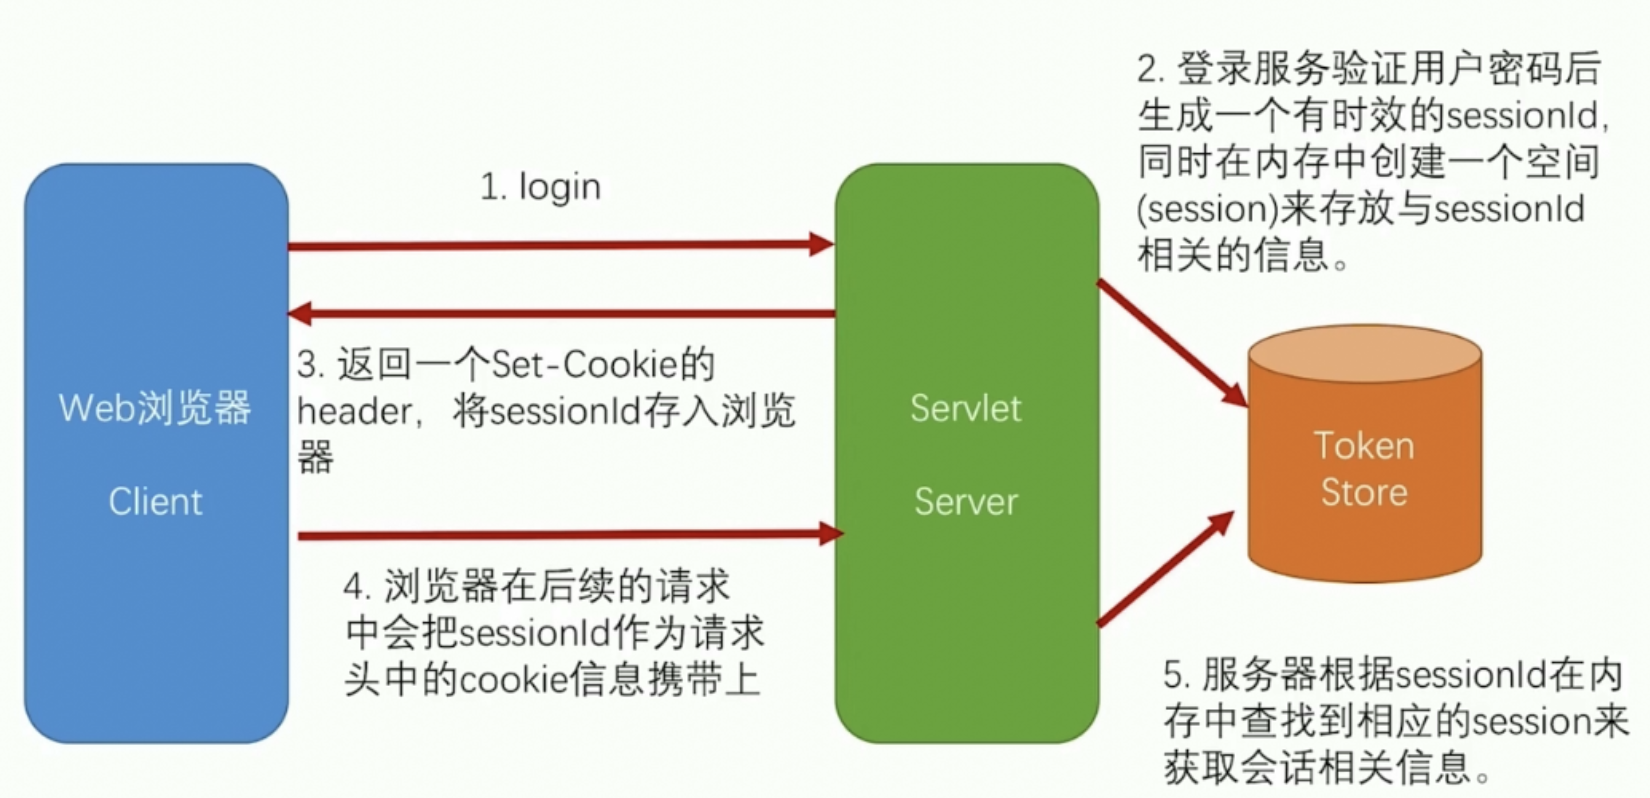
\includegraphics[scale=0.5]{resources/img/i25.png}
  \caption{HTTP请求返回验证Cookie示意图}
\end{figure} 
图5.10为HTTP请求返回验证Cookie流程。
我们可以得出结论:
只要得到了别的客户端的cookie,我们就可以假冒成它来和服务器对话。这给我们的程序带来了可乘之机。
我们先用抓包工具开始抓包HTTP请求,然后使用抓包工具的开发者工具查看cookie。
接着在抓包工具复制对应的HTTP请求头数据携带该cookie在程序中发送HTTP请求,
就能让程序伪装APP通过改变参数发出特定的请求操作。
\newline
下面我们开始通过抓包流量进行分析,我们有两种方法搭载热点:a.使用一个普通的
无线路由器作为无线热点;b.使用无线网卡连接笔记本电脑,配置一个无线热点。对
于这两种搭建无线局域网的方式,我们使用不同的方法进行抓包分析。
这里我们采用Fiddler\cite{crane2015fiddler}这款软件来进行数据抓取, Fiddler不仅可以抓web页面的HTTP/HTTPS的数据报文, 也可以抓取我们手机移动端的数据报文。
在攻击目标与服务器之间充当中间人的角色,嗅探两者之间的数据流量,从而窃取用户的数据资料。
前提条件是手机必须处于同一个网络当中, 并且手机网络代理必须设置为fiddler,当我们的手机经过Fiddler这一层服务。
具体步骤如下:
\begin{itemize}
    \item 确保手机和PC在同一网络环境下,让手机和fiddler在同一局域网下。
    \item 让android手机的网络进出口指向局域网中fiddler服务地址, 那么我们这里就必须要知道Fiddler的ip地址和端口号(port), 这里Fiddler的ip地址就是我们当前电脑中的本机ip地址
    \item Fiddler设置端口与允许远程连接 在Fiddler中我们还要设置远程连接权限和端口号, 找到Fiddler菜单栏中的Tools ----> Options---->Connections, 勾选Allow remote computers to connect(允许远程计算机连接) 然后设置一个端口,也可以默认为8888。 以上所有Fiddler设置之后最好是重启一下Fiddler,才可以让配置生效。
    \item android手机设置网络代理 在确定了手机和fiddler在同一局域网下之后, 那么我们来到android手机的设置选项下,找到WLAN 改成IP手动代理模式 对应IP为Fiddler的ip地址和端口
    \item android手机配置证书 在抓取android手机数据包的时候 跟 web端也是一样,都需要配置证书,否则是无法正常进行抓包的。之前已经在我们的android手机上配置好了Fiddler的代理服务了,那么现在就可以通过ip+port的方式来访问Fiddler 从而下载对应的证书。
\end{itemize}

在设置好了Fiddler之后,我们通过车联网APP进行了查看车辆信息(车辆四门开关状态、行驶里程、剩余流量、续航里程、发动机状态)的操作与此同时APP发起了HTTP请求,通过Fiddler我们
成功了侦测到了该请求以及返回数据。如图所示:
\begin{figure}
  \centering
  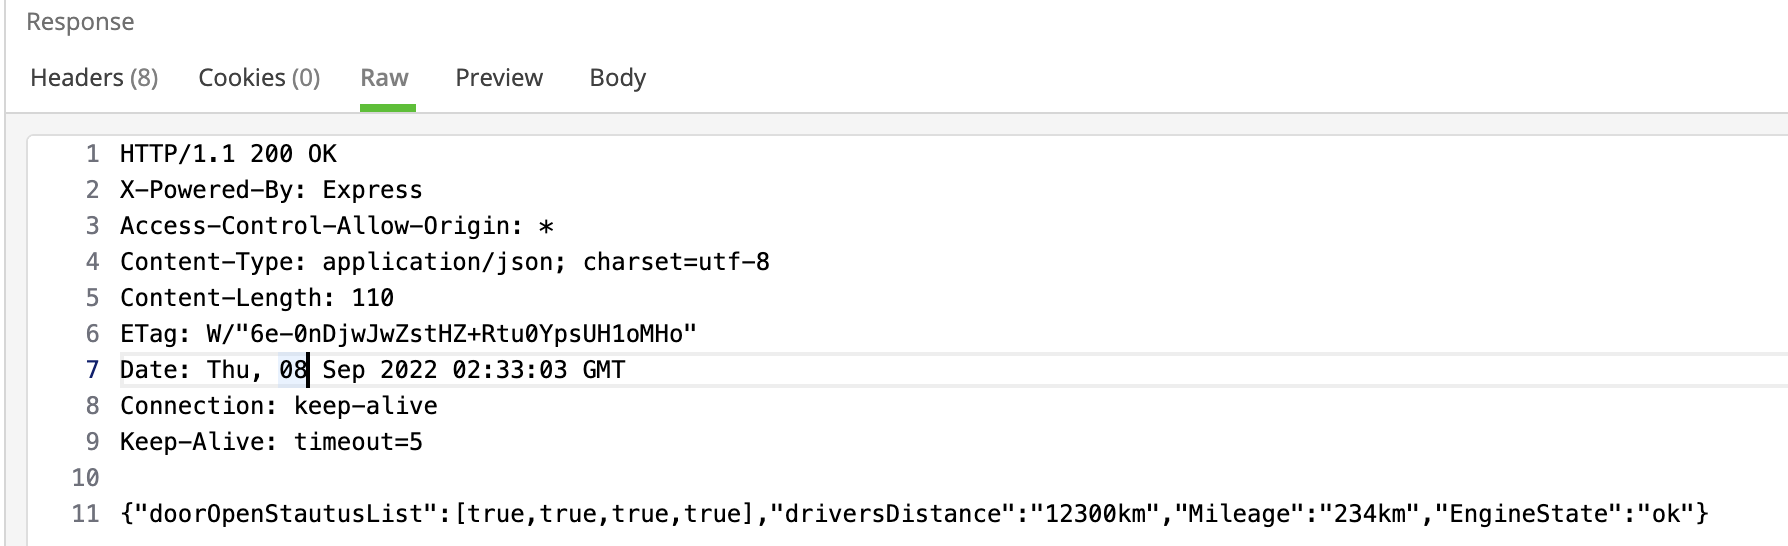
\includegraphics[scale=0.5]{resources/img/i26.png}
  \caption{Fiddler抓取HTTP请求车辆状态信息接口图}
\end{figure}
我们发现手机APP有控制车门开关功能,因此我们通过手机APP点击关门,此时Fiddler也同样侦测到了请求
如法炮制我们利用Fiddler中的Composer功能自定义服务请求发送到服务器,
可以手动创建一个新的请求,也可以在会话表中,拖拽一个现有的请求并进行修改;
因此Composer可以篡改Cookie中的数据。也就是说,Inspectors篡改的是我们输入的数据,这里类似Web安全中CSRF请求攻击\cite{blatz2007csrf},
主要操作步骤如下:
\begin{itemize}
  \item 首先定位到那条开车门请求记录,然后用鼠标将该条请求记录的位置拖拽到Composer中接口。Composer会自动读取到该条请求的所有数据。
  \item 篡改数据。直接在Composer中的Request Body或者是请求头信息中修改数据
  \item 点击“Execute”按钮执行发送请求。
\end{itemize}
由于"开门"“关门”操作是同一个HTTP请求接口只是参数不同,因此我们可以任意的篡改参数任意实现开关门。

\section{本章小结}
本章主要描述针对一款实际商用的汽车进行渗透攻击的实验。先从攻击模型入
手,在第四章进行威胁建模的基础上,搭建攻击环境;然后进行蓝牙近距离通信伪造操作请求 成功的发送伪造请求 解锁了车辆车门;接着对汽车搭配的远
程控制 App 进行逆向操作,从汇编源码找到部分关键逻辑,编写攻击的软件,成功
获取车主隐私信息和车辆状态信息;最后我们通过抓包手机互联APP发送的汽车操作HTTP请求获得了登录凭证Token
通过该凭证我们实现了伪造请求远程操控智能网联汽车的入侵行为。
